\section{Proceso de Poisson}
\label{procPoisson-chapter}
En este capítulo estudiaremos uno de los procesos más importantes para nuestro modelo matemático: el proceso de Poisson. Definiremos este proceso de varias formas equivalentes y estudiaremos algunas de sus propiedades, generalizaciones y algunas de sus aplicaciones.
\subsection{Definición constructiva}
    Suponga que un mismo evento ocurre repetidas veces de manera aleatoria a lo largo del tiempo.\\
    Tal evento puede ser la recepción de una llamada, la llegada de un cliente a una ventanilla para solicitar algún servicio o los momentos en que una cierta maquinaria requiere reparación, etc.\\
    \begin{Def}(\textit{Primera definición})
        Sea $T_1$, $T_2, \ldots T_n$ una sucesión de variables aleatorias independientes cada una con distribución distribución exponencial de parámetro $\lambda>0$. Un proceso estocástico a tiempo continuo $\{X_t\}_{t\geq 0}$ definido como
        \begin{eqnarray}
            X_t = \max \{ n\in\N : T_1+T_2+\cdots+T_n \leq t\}
            \label{def-formula-constructiva-poisson}
        \end{eqnarray}
        es llamado proceso de Poisson de parámetro $\lambda$ homogéneo.
        Se postula además que el proceso debe iniciar en cero ( $t=0$) y para ello se define $\max \phi=0$.\\
        De forma intuitiva, la variable $X_t$ expuesto en \ref{def-formula-constructiva-poisson}  equivale a contar el número de eventos ocurridos durante el tiempo $t$. Es decir.
        $$X_t = \textit{ `Número de ocurrencias al tiempo $t$'}$$
        \label{def-procesoPoison-constructiva}
    \end{Def}
    A los tiempos $T_1 ,\thinspace T_2,\thinspace\ldots$ se los llama tiempos de estancia y corresponden a los tiempos que transcurren entre un salto del proceso y el siguiente salto.\\
    Una de las características sobresalientes de este proceso es que puede encontrarse explícitamente la distribución de la probabilidad de la variable $X_t$ para cualquier valor de $t\geq 0$, la cual coincide con la distribución de Poisson, y de allí es de donde el proceso adquiere su nombre.
    \begin{Prop}
        Dado $t\geq 0$, la variable aleatoria $X_t$ tiene distribución Poisson con parámetro $\lambda t$.
    \end{Prop}
   \begin{Cor}
   Sea $\{X_t\}_{t\geq 0}$ un proceso de Poisson, entonces para cada $t\geq 0$ , $$E(X_t)=\lambda t,$$ en particular, 
   $$E(X_1)=\lambda$$
   
   \end{Cor}
   Esto nos muestra que la variable $\lambda$ se interpreta con la cantidad media o esperanza de que en un intervalo haya algún cambio .\\
   Una de las propiedades que caracterizan de manera única a la distribución exponencial dentro del conjunto de distribuciones absolutamente continuas es que satisface la propiedad de pérdida de memoria, esto es, si $T$ tiene distribución exponencial de parámetro $\lambda$, entonces para cualesquiera tiempos $s$, $t\geq$ se cumple la igualdad $$P(T>t+s|\thinspace T>s)=P(T>t).$$
    En otras palabras, condicionada al evento $(T>s)$, la variable $(T-s)$ sigue teniendo distribución exponencial con parámetro $\lambda$.
    Esto significa que, para un valor de $s\geq 0$ fijo, todos los tiempos de estancia a partir de $s$, incluyendo el primero, siguen teniendo distribución exponencial $\lambda$, y por lo tanto el proceso de conteo de eventos a partir del tiempo $s$ es un proceso de Poisson.
    \begin{Prop} 
        El proceso de Poisson $\{X_t\}_{t\geq 0}$ satisface las siguientes
        propiedades.
        \label{prop_procPoisson_constructiva}
        \begin{enumerate}[a)]
            \item  Es un proceso de Markov.
            \item Tiene incrementos independientes.
            \item Tiene incrementos estacionarios.
            \item Para cualesquiera $s,t \geq 0$ y los enteros $0\leq i\leq j$ las probabilidades de transición son, $$P(X_{t+s}=j\thinspace|\thinspace X_s=i)= e^{-\lambda t}\frac{(\lambda t)^{j-i}}{(j-i)!}$$
            \item Para cualesquiera tiempos $0\leq s\leq t$, y para $n=0,1,\ldots$
            $$P(X_t-X_s=n)=P(X_{t-s})$$
        \end{enumerate}
    \end{Prop}
    La definición de proceso de Poisson es constructiva pues a partir de los
    tiempos de estancia se construye el proceso de conteo correspondiente.\\
    Existen otras formas equivalentes y un tanto axiomáticas de definir a este
    proceso.\\
    Una de las ventajas de contar con estas definiciones alternativas es que para demostrar que un cierto proceso es de Poisson se puede tomar cualquiera de las definiciones a conveniencia.\\
\subsection{Definición infinitesimal}
    Sea $S=\{0,\thinspace 1,\thinspace 2,\ldots\}$ un conjunto de estados.\\Se denota $P_n(t)$ como la probabilidad de que en el tiempo $t$ sucedan $n$ ocurrencias nuevas.\\
    \begin{Obs}
    Haremos uso del término 'época' para denotar puntos en el eje de tiempo y la palabra 'tiempo' se referirá a duraciones ( o longitudes de los intervalos entre las épocas).
    \end{Obs}
    Para deducir esto, primero se divide un intervalo de tiempo de longitud unitaria en $N$ subintervalos de longitud $h=N^{-1}$.
    La probabilidad de que en algún subintervalo de longitud de tiempo $h$ no tenga lugar alguna ocurrencia es denotada por $P_0(h)$. 
    Esto puede ser el caso de que en un tiempo $t$ el proceso se encuentre en un estado $n$ y al cabo de $h$ de tiempo, el proceso siga en ese estado, sin producirse ningún cambio. Esto implica que la probabilidad de que ocurra al menos un cambio en el intervalo $[t,t+h)$ es de  $1-P_0(h)$, y de esta manera el número esperado de subintervalos en las que suceda al menos una ocurrencia será $N\cdot(1-P_0(h))=h^{-1}(1-P_0(h))$.
    \\Si, por ejemplo, se divide el intervalo unitario en $N=10$ subintervalos de longitud $h=0.1$ cada uno, representado en la figura (\ref{fig-procesoPoison-recta1}). Los puntos sobre la recta representan los diversos sucesos $S_i,\thinspace i=1,2,\ldots,10$ que se puedan presentar en ese intervalo unitario de tiempo.\\ Como se puede observar, hay subintervalos que albergan más de un suceso.
    \begin{center}
        \begin{figure}[htb]
            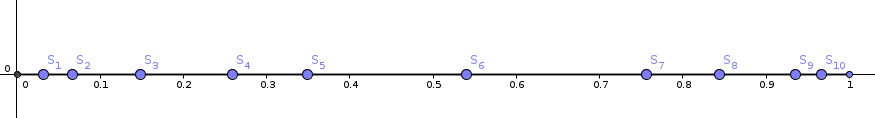
\includegraphics[width=14cm]{Cap2-ProcesosEstocásticos/img/recta1.png}
            \caption{Intervalo unitario dividido en 10 subintervalos.}
            \label{fig-procesoPoison-recta1}
            \vspace*{0.05in}
        \end{figure}
    \end{center}
    Si se divide el intervalo en $N=20$ subintervalos de longitud $h=0.05$, se aprecia que cada uno contiene un suceso o no contiene ninguno ( Ver figura \ref{figurarecta2} )\\  
    \begin{center}
        \begin{figure}[htb]
           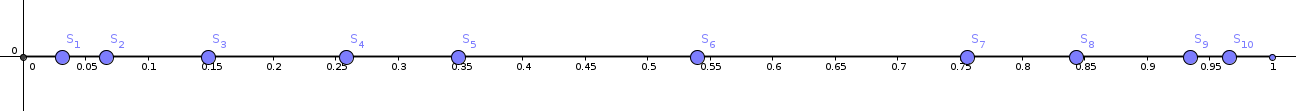
\includegraphics[width=14cm]{Cap2-ProcesosEstocásticos/img/recta2.png}
           \caption{Intervalo unitario dividido en 20 subintervalos.}
        \label{figurarecta2}
        \vspace*{0.05in}
        \end{figure}
    \end{center}
    La probabilidad de que no suceda un cambio en todo el intervalo unitario gracias a la probabilidad clásica definida será $P_0(1)=\frac{10}{20}=0.5$ entonces $\frac{1-P_0(h)}{h}=\frac{1-0.5}{0.05}=10$ que justamente coincide con el total de sucesos.\\
    Intuitivamente, cuando los subintervalos se vuelven suficientemente pequeños $(h\rightarrow 0)$ de tal forma que cada uno contenga a lo mucho un suceso, este numero converge al número esperado de saltos dentro del intervalo unitario que es número finito $\lambda$, la cual se interpreta como la media, esperanza o número medio de ocurrencias en el intervalo de tiempo unitario.
    Esto es
    $$  \lim_{h\rightarrow 0}\frac{1-P_0(h)}{h}=\lambda
    $$
  
    %%%%%%%%%%%%%%%%%%%%%%%%%%%%%%%%%%%%%%%%%%%%%%%%%
    \begin{comment}
    $X([a,b])$ es el número de ocurrencias en el intervalo $[a,b]$, sean $w_i$ el tiempo de espera antes de que pase una ocurrencia adicional después de la $i$-ésima ocurrencia.
    Dado $\epsilon>0$, se toma $\delta=\min\{w_i, i=1,2,\ldots,\lambda\}$, si $|h|<\delta$ , $X([(i-1)h,ih])$, $i=1,2,\ldots\lambda$ a lo mucho puede ser 1. entonces $1-P_0(h)=P_1(h)$ $|\frac{(1-P_0(h))}{h}-\lambda|=|N(P_1(h))-\lambda|=|N\frac{\lambda}{N}-\lambda|=0<\epsilon $, esto es:
    \end{comment}
    %%%%%%%%%%%%%%%%%%%%%%%%%%%%%%%%%%%%%%%%%%%%%%%%%
    La cual también puede ser escrita como $o(h)+1-P_0(h)=\lambda h$, donde $o(h)$ denota una cantidad que cumple que $\lim_{h\rightarrow 0}\frac{o(h)}{h}=0$. Como consecuencia se tiene
    \begin{eqnarray}
        P_0(h)=1-\lambda h+o(h)
        \label{procesoPoison-cond1}
    \end{eqnarray}
    Cuando el intervalo de tiempo es extremadamente pequeño la probabilidad de que suceda más de una ocurrencia, es nula, pues cada subintervalo contiene a lo mucho un suceso. Esto es,
    \begin{eqnarray}
        P_n(h)=o(h),\quad n\geq 2
        \label{procesoPoison-cond2}
    \end{eqnarray}
    $$\lim_{h\rightarrow 0}\frac{1-P_0(h)-P_1(h)}{h}=0$$
    o lo que es lo mismo $1-P_0(h)-P_1(h)+o(h)=0$, de donde, se obtiene que
    \begin{eqnarray}
        P_1(h)=\lambda h+o(h)
         \label{procesoPoison-cond3}
    \end{eqnarray}
    \begin{Def}(Definición infinitesimal)\\
         El proceso estocástico $\{X_t\}_{t\geq 0}$
        descrito con las características (\ref{procesoPoison-cond1}), (\ref{procesoPoison-cond2}), (\ref{procesoPoison-cond3}), con incrementos independientes y estacionarios, y $X_0=0$ es llamado un proceso de Poisson.
    \end{Def}
    Esta definición hace uso de las probabilidades infinitesimales del proceso y ello tiene algunas ventajas desde el punto de vista de la interpretación de
    lo que sucede en un intervalo infinitesimal de tiempo $[t,t+h)$.
    \begin{Prop}
        El proceso de Poisson $\{X_t\}_{t\geq 0}$ descrito con la definición infinitesimal tiene distribución de Poisson con parámetro $\lambda t.$ Esto es,
        $$P_n(t)=\frac{(\lambda t)^n}{n!}e^{-\lambda t}, \quad n\in\N$$
    \end{Prop}
    \begin{proof}
        Dado $n\in\N$, analicemos la probabilidad para un tiempo $t+h$, donde el sistema se encuentre en estado $n$ $(X_{t+h}=n)$. Esto puede ocurrir solo de tres maneras independientes.
        \begin{itemize}
            \item SITUACIÓN A: En el tiempo $t$ el sistema estaba en el estado $n$ y no ocurre ningún cambio. $A=(X_t=n,\thinspace X_{t+h}=n)$, entonces la probabilidad que suceda esta situación estará dada por $$P(A)=P(X_t=n,\thinspace X_{t+h}=n)=P(X_t=n)P(X_{t+h}=n|\thinspace X_{t}=n)=P_n(t)P_0(h)$$\\
            Por la condición (\ref{procesoPoison-cond1})
            tenemos que:
            $$P(A)=P_n(t)(1-\lambda h)+o(h)$$
            \item SITUACIÓN B: En la época $t$ el sistema se encontraba en el estado $n-1$ y ocurre tan solo un cambio. Se tiene que $B=(X_{t+h}=n, X_t=n-1)$ ,entonces la  probabilidad que suceda eso estará dada por
            $$P(B)=P(X_{t+h}=n, X_t=n-1)=P(X_t=n-1)P(X_{t+h}=n|X_t=n-1)P_{n-1}(t)P_1(h)$$
             Por la condición (\ref{procesoPoison-cond3})
            tenemos que:
            $$P(B)=P_n(t)(\lambda h)+o(h)$$
            \item SITUACIÓN C: En la época t el sistema estaba en el estado n-1 y ocurrió más de un cambio.
            $$P(C)=P(X_{t+h}=n, X_t=n-k)=P_n(t)P_k(h), \quad k\geq 2$$
             Por la condición (\ref{procesoPoison-cond2})
            tenemos que
            $$P(C)=o(h)$$
        \end{itemize}
        Por la definición de las situaciones $A$, $B$ y $C$ forman una partición de $(X_{t+h}=n)$ pues su intersección es nula y la unión de ellos nos da el espacio muestral completo $(X_{t+h}=n)$. Como consecuencia 
        $$P_n(t+h)=P(A\cup B\cup C=P(A)+P(B)+P(C)$$ $$=(1-\lambda h)P_n(t)+\lambda h P_{n-1}(t)+o(h)$$
        $$\frac{P_n(t+h)-P_n(t)}{h}=-\lambda P_n(t)+\lambda P_{n-1}(t)+\frac{o(h)}{h}$$
        Finalmente, cuando $h\rightarrow 0$
        \begin{eqnarray}
            \begin{cases}
                P'_n(t)=-\lambda P_n(t)+\lambda P_{n-1}(t),\quad n\geq 1\\
                P_n(0)=0
            \end{cases}
            \label{ProcPoison-edo-n}
        \end{eqnarray}
        Cabe resaltar que cuando $t=0$ nunca ocurre algún cambio pues no ha transcurrido ningún tiempo aún. Por ello $P_0(0)=1$ y $P_n(0)=0$, $n\in\N$. \\
        Ahora, para el caso particular de $n=0$.\\
        $$P_0(t+h)=P_0(t)P_0(h)=P_0(t)(1-\lambda h)+o(h)$$
        entonces
        \begin{eqnarray}
            \begin{cases}
                P'_0(t)=-\lambda P_0(t)\\
                P_0(0)=1
            \end{cases}
             \label{ProcPoison-edo-0}
        \end{eqnarray}
        Resolviendo la ecuación diferencial \ref{ProcPoison-edo-0} se tiene $P_0(t)=e^{-\lambda t}$.\\
        Como $P_n$ está definida recursivamente para $n\in\N$ usando inducción,
        para $n=1$ tenemos 
        $$\begin{cases}
            P'_1(t)=-\lambda P_1(t)+\lambda e^{-\lambda t}\\
            P_1(0)=0
        \end{cases}$$
        Usando el método de factor integrante se tiene que $P_1(t)=\lambda te^{-\lambda t}$
        \\Nuestra hipótesis inductiva es 
        $P_n(t)=\frac{(\lambda t)^n}{n!}e^{-\lambda t}$
        Entonces 
        $$\begin{cases}
            P'_{n+1}(t)=-\lambda P_{n+1}(t)+\frac{(\lambda t)^n}{n!}e^{-\lambda t}\\
            P_{n+1}(0)=0
        \end{cases}$$
        Usando nuevamente el método de factor integrante se tiene que
        $$P_{n+1}(t)=\frac{(\lambda t)^{n+1}}{n+1!}e^{-\lambda t}$$
        Lo cual prueba el resultado.
    \end{proof}
    Con esta notación, las probabilidades encontradas se las conocen como postulados de Poisson.\\
    Estas condiciones son débiles puesto que da entender que para cada suceso, la media o esperanza $\lambda$ del número de ocurrencia se mantiene constante durante todo el proceso sin importar en qué estado se encontraba previamente.\\
    Esto es, para dado $n\in\N$,  $P_{i-1,i}(h)=P_{j-i,j}(h)=\lambda h + o(h)$ para cualquier $j,i=0,\thinspace 1,\thinspace 2 ,\ldots$ lo cual no siempre sucede en la vida real.
    \\He ahí la importancia de introducir una noción más generalizada.